\chapter{Ограниченная струна. Метод Фурье.}
\label{cha:9}

\section*{Правило параллелограмма}

\begin{remem}

	\begin{multicols}{2}
		\begin{flushleft}
			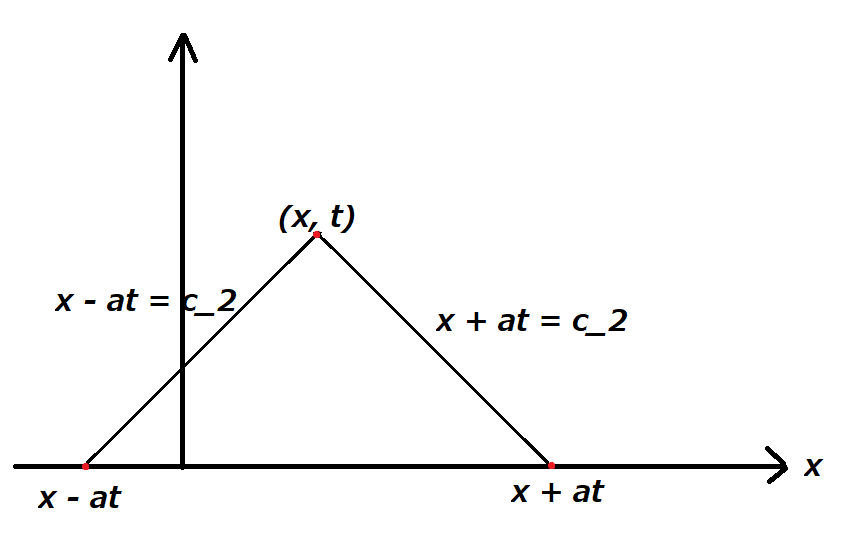
\includegraphics[scale=0.4]{char_triangle} 
		\end{flushleft}

		\columnbreak

		\hfill \break \hfill \break \hfill \break
		$$\begin{cases}
			u_{tt} = a^2 u_{xx}, \; t > 0, \; x \in \mathbb{R} \\
			u|_{t = 0} = \varphi (x) \\
			u_t |_{t = 0} = \psi (x)
		\end{cases}$$
	\end{multicols}

	\textit{Общее решение}: $ u(t, x) = f(x - at) + g(x + at). $ Значение функции в точке $ (t, x) $ зависит от $ x \pm at $, не зависит от точек вне отрезка $ [x - at, x + at] \; \Rightarrow $  боковые стороны треугольника - характеристики. Треугольник называется \red{характеристическим}.
\end{remem}

\begin{clair}[\blue{Правило параллелограмма}]
	Для описанной функции $u$ справедливо следующее равенство: $ u(A) + u(C) = u(B) + u(D) = 0 $.
	\begin{center}
		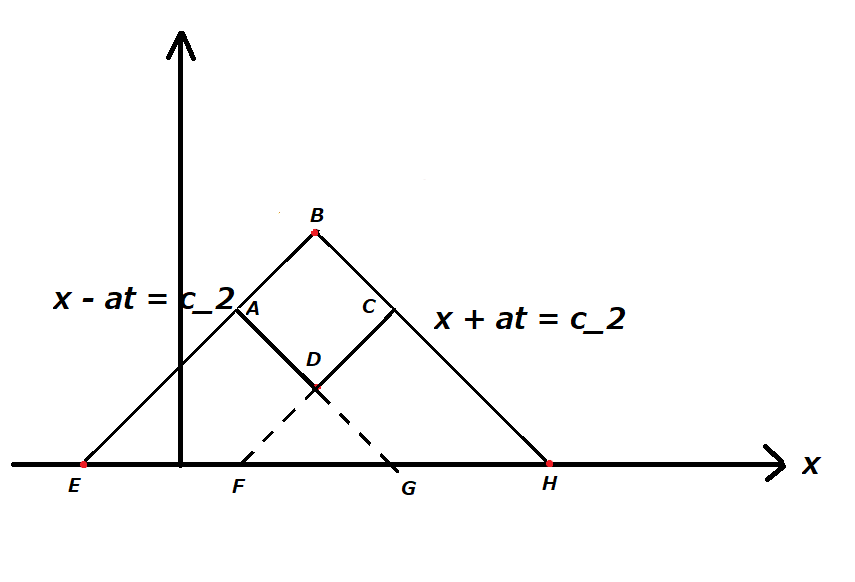
\includegraphics[scale=0.4]{triag_proof}
	\end{center}
\end{clair}
\begin{Proof}
	По формуле Д'Аламбера: 
	$$\begin{gathered}
		u = \dfrac{1}{2}(\varphi(x - at) + \varphi(x + at)) + \dfrac{1}{2a} \int\limits_{x - at}^{x + at} \psi(y)dy
	\end{gathered}$$
	Тогда получаем следующие значения функции в точках:
	$$\begin{gathered}
		u(A) = \dfrac{1}{2}(\varphi(E) + \varphi(G)) + \dfrac{1}{2a} \int\limits_{E}^{G} \psi(y)dy, \; u(C) = \dfrac{1}{2}(\varphi(F) + \varphi(H)) + \dfrac{1}{2a} \int\limits_{F}^{H} \psi(y)dy \\
		u(B) = \dfrac{1}{2}(\varphi(E) + \varphi(H)) + \dfrac{1}{2a} \int\limits_{E}^{H} \psi(y)dy, \; u(D) = \dfrac{1}{2}(\varphi(F) + \varphi(G)) + \dfrac{1}{2a} \int\limits_{F}^{G} \psi(y)dy
	\end{gathered}$$
\end{Proof}

Рассмотрим следующую задачу:
\begin{multicols}{2}
	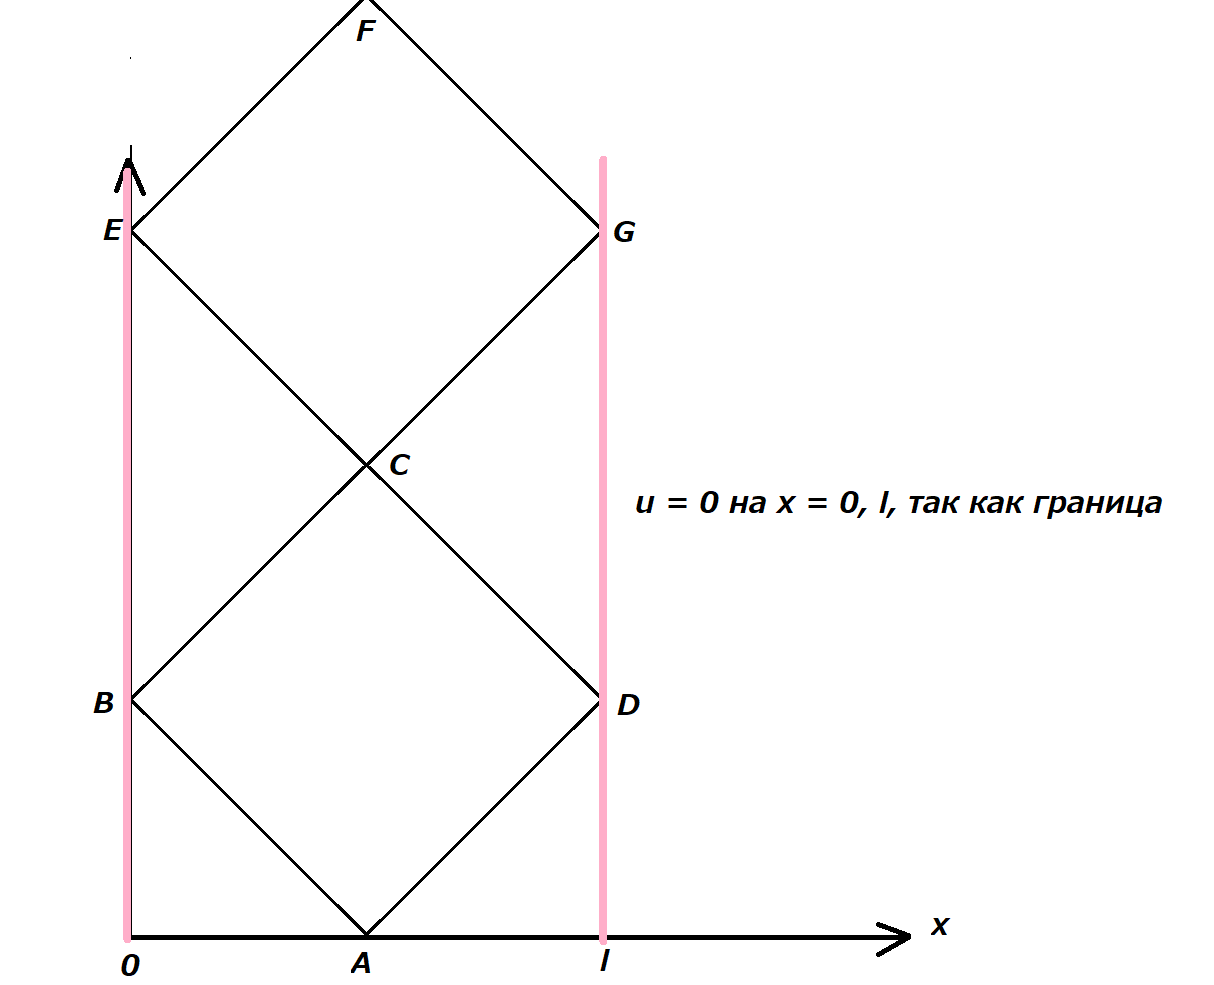
\includegraphics[scale=0.3]{paral}
	\columnbreak
	$$\begin{cases}
		u_{tt} = a^2 u_{xx}, \; t > 0, \; x \in (0, l) \\
		u|_{t = 0} = \varphi (x) \\
		u_t |_{t = 0} = \psi (x) \\
		u|_{x = 0} = 0 \\
		u|_{x = l} = 0
	\end{cases}$$

	\hfill \break 
	По правилу параллелограмма получаем:
	$$\begin{gathered}
		u(A) + u(C) = u(B) + u(D) = 0 \\
		u(C) + u(F) = u(G) + u(E) = 0
	\end{gathered}$$
\end{multicols}

Таким образом получаем, что $u(A) = -u(C)$ и $-u(C) = u(F)$. Абсцисса точки $A$ совпадает с абсциссой точки $F$, значит функция периодическая. Найдем период:
$$l = \dfrac{T}{2}a \; \Rightarrow \;  T = \dfrac{2l}{a}, \; u(t, x) = u(t + \dfrac{2l}{a}, x)$$
\newpage

\section*{Ряд Фурье}

Пусть $x \in (0, l)$ и $X_n(x) $ - базис, т.е. $ (X_n, X_m ) = \int\limits_{0}^l X_n(x)X_m(x) dx = 0$ при $n \ne m $.

Рассмотрим представление функции в виде \textit{ряда Фурье}: $f(x) = \sum\limits_{n = 0}^\infty f_n(x)X_n(x)$.
Найдем $f_k$, скалярно домножив на $X_k$:
$$\begin{gathered}
	f(x) = \sum\limits_{n = 0}^\infty f_n(x)X_n(x) \; \; \Big| \cdot X_k \\
	(f(x), X_k) = f_k(x)||X_k||^2 \; \Rightarrow \; f_k(x) = \dfrac{(f(x), X_k)}{(X_k, X_k)}
\end{gathered}$$
Будем искать решение $ u(t, x) $ в виде ряда: $u(t, x) = \sum\limits_{n = 0}^\infty T_n(t)X_n(x)$.

\begin{enumerate}
	\item 
		Найдем базис. Введем вспомогательную функцию $ v(t, x) = T(t)X(x) \not\equiv 0 $ -- одно слагаемое ряда.
		$$\begin{gathered}
			\begin{cases}
				v_{tt} = a^2v_{xx}, \; t > 0, \; x \in (0, l) \\
				v|_{x = 0} = 0 \\
				v|_{x = l} = 0 \\
			\end{cases} \Rightarrow \begin{cases}
				T''(t)X(x) = a^2T(t)X''(x) \\
				T(t)X(0) = 0\\
				T(t)X(l) = 0
			\end{cases} \Rightarrow \\
			\Rightarrow \; \dfrac{T''(t)}{T(t)a^2} = \dfrac{X''(x)}{X(x)} = -\lambda = const \; \Rightarrow \begin{cases}
				X''(x) + \lambda X(x) = 0 \\
				X(0) = 0\\
				X(l) = 0
			\end{cases}
		\end{gathered}$$

		\section*{Задача Штурма - Луивилля}

		\textit{Задача Штурма - Луивилля} -- задача на отыскание нетривиальных собственных функций и собственных значений оператора.

		\begin{itemize}
			\item 
				$ \lambda = 0 \; \Rightarrow \;  X(x) = c_1x + c_2 \equiv 0$.\\
				В силу дополнительных условий $\lambda $ - не собственное значение.
				\hfill \break
			\item  
				$ \lambda < 0 \; \Rightarrow \;  X(x) = c_1e^{x\sqrt{-\lambda}} + c_2e^{-x\sqrt{-\lambda}}$.\\
				В силу дополнительных условий $ c_1 = c_2 = 0 \; \Rightarrow \;  \lambda $ - не собственное значение.
				\hfill \break
			\item 
				$ \lambda > 0 \; \Rightarrow \;  X(x) = c_1\sin(x\sqrt{\lambda}) + c_2\cos(x\sqrt{\lambda})$.\\ 
				В силу дополнительных условий $ c_2 = 0, \; c_1\sin(\sqrt{\lambda}l) = 0 \; \Rightarrow$

				$\Rightarrow \; \sqrt{\lambda}l = \pi n, \; n \in \mathbb{Z} \; \Rightarrow \; \lambda = \dfrac{\pi^2n^2}{l^2}, \; n \in \mathbb{Z} \; \Rightarrow$

				$\Rightarrow \begin{cases}
					X_n(x) = c_1 \sin(\frac{\pi n}{l}x), \; n = 1, 2, \dots \\
					X_0 = 0 \\
					n < 0 \text{ не подходят, так как } \sin(x) \text{ - нечетная функция}
				\end{cases}$

				Пусть $ c_1 = 1 \; \Rightarrow \; X_n(x) = \sin(\frac{\pi n}{l}x), \; n = 1, 2, \dots$
		\end{itemize}

	\item 
		Найдем коэффициенты $ T_n(t). \; u(t, x) = \sum\limits_{n = 1}^\infty T_n(t)\sin(\frac{\pi n}{l}x) \; \Rightarrow$
		$$\begin{gathered}
			\Rightarrow \begin{cases}
				\sum\limits_{n = 1}^\infty T_n''(t)\sin(\frac{\pi n}{l}x) = 
				-\dfrac{a^2\pi^2n^2}{l^2}\sum\limits_{n = 1}^\infty T_n(t)\sin(\frac{\pi n}{l}x)\\
				\sum\limits_{n = 1}^\infty T_n(0)\sin(\frac{\pi n}{l}x) = \varphi(x) \\
				\sum\limits_{n = 1}^\infty T_n'(0)\sin(\frac{\pi n}{l}x) = \psi(x)
			\end{cases} \\
			\varphi(x) = \sum\limits_{n = 1}^\infty \varphi_n\sin(\frac{\pi n}{l}x), \; \varphi_n = \dfrac{(\varphi(x), X_n(x))}{(X_n(x), X_n(x))} \;\Big(\text{аналогично для } \psi(x) \Big)
		\end{gathered}$$
		Имеем систему:
		$$\begin{gathered}
			\begin{cases}
				T_n''(t) = -(\dfrac{a\pi n}{l})^2T_n(t) \\
				T_n(0) = \varphi_n \\
				T_n'(0) = \psi_n
			\end{cases} \Rightarrow 
			\begin{cases}
				T_n(t) = A_n \sin(\frac{a \pi n}{l}t) + B_n \cos(\frac{a \pi n}{l}t) \\
				T_n(0) = B_n = \varphi_n \\
				T_n'(0) = \dfrac{a \pi n}{l} A_n = \psi_n
			\end{cases}
		\end{gathered}$$
		Итоговая формула имеет вид:
		$$T_n(t) = \psi_n \dfrac{ l}{a \pi n} \sin(\frac{a \pi n}{l}t) + \varphi_n \cos(\frac{a \pi n}{l}t) $$
\end{enumerate}
	
\section*{Метод Фурье: общий случай}
	
$$\begin{cases}
	u_{tt} = a^2 u_{xx} + f(x), \; t > 0, \; x \in (0, l) \\
	u|_{t = 0} = \varphi (x) \\
	u_t |_{t = 0} = \psi (x) \\
	(\alpha u_x - \beta u)|_{x = 0} = \mu(t) \\
	(\gamma u_x - \delta u)|_{x = l} = \nu(t)
\end{cases}$$

\begin{enumerate}
	\item 
		Сделаем граничные условия однородными. Введем вспомогательную функцию $ \omega(t, x): $
		$$\begin{cases}
			(\alpha \omega_x - \beta \omega)|_{x = 0} = \mu(t) \\
			(\gamma \omega_x - \delta \omega)|_{x = l} = \nu(t)
		\end{cases}\eqno(*)$$
		Допустим, что такая функция найдена. Пусть $ z = u - \omega$, тогда $u = z + \omega$ и наша задача для функции $z$ имеет вид:
		$$\begin{cases}
			z_{tt} = a^2 z_{xx} + f(x), \; t > 0, \; x \in (0, l) \\
			z|_{t = 0} = \varphi_1 (x) \\
			z_t |_{t = 0} = \psi_1 (x) \\
			(\alpha z_x - \beta z)|_{x = 0} = 0 \\
			(\gamma z_x - \delta z)|_{x = l} = 0
		\end{cases}$$
		\begin{itemize}
			\item 
				если 
				$\left[
					\begin{gathered}
						\alpha = 0, \gamma = 0 \\
						\alpha = 0, \; \delta = 0 \\
						\beta = 0, \; \gamma = 0
					\end{gathered}
				\right.$, то $\omega = g(t)x + c(t)$
			\item 
				если $\beta = 0, \; \delta = 0$, то $\omega = d(t)x^2  + g(t)x + c(t)$

			(коэффициенты $ d(t), g(t), c(t) $ находятся из условия $ (*) $)
		\end{itemize}
	\item 
		Свели задачу к задаче с однородными граничными условиями. Пусть $ u = z $. Знаем, что $f(x) = \sum\limits_{n = 0}^\infty f_n(x)X_n(x), \; f_k(x) = \dfrac{(f(x), X_k)}{(X_k, X_k)}$.\\
		Тогда здача Коши для $ T_n(t) $ примет вид:
		$$\begin{cases}
			T_n''(t) = -(\dfrac{a\pi n}{l})^2T_n(t) + f_n(t)\\
			T_n(0) = \varphi_n \\
			T_n'(0) = \psi_n
		\end{cases}$$
\end{enumerate}

\section*{Базисы в зависимости от граничных условий на х}
\begin{multicols}{2}
	$\begin{cases}
		X(0) = 0 \\
		X(l) = 0
	\end{cases} 
	X_n(x) = \sin(\frac{\pi n}{l}x)$

	\columnbreak

	$\begin{cases}
		X(0) = 0 \\
		X'(l) = 0
	\end{cases}
	X_n(x) = \sin(\frac{\pi}{l}(n + \frac{1}{2})x)$
\end{multicols}

\begin{multicols}{2}
	$\begin{cases}
		X'(0) = 0 \\
		X'(l) = 0
	\end{cases} 
	X_n(x) = \cos(\frac{\pi n}{l}x)$

	\columnbreak
	
	$\begin{cases}
		X'(0) = 0 \\
		X(l) = 0
	\end{cases}
	X_n(x) = \cos(\frac{\pi}{l}(n + \frac{1}{2})x)$
\end{multicols}
	
	
	
	
	
	
	
	